
\documentclass[twocolumn]{aastex6}

\bibliographystyle{aasjournal}
\usepackage{graphicx}
\usepackage[suffix=]{epstopdf}
\usepackage{natbib}
\usepackage{amsmath}
\usepackage{url}
\usepackage{xspace}

%    Make Scientific Notation
\providecommand{\e}[1]{\ensuremath{\times 10^{#1}}}

% make the word Kepler italicized
\newcommand{\Kepler}{\textsl{Kepler}\xspace}



\begin{document}
%%%%%%%%%%%%%%%%%%%%%%
\title{Stellar Flares and the Age-Activity Relationship}

\shorttitle{Flares }
\shortauthors{Davenport et al.}

\author{
	James R. A. Davenport\altaffilmark{1,2,3},
	Marcel Ag\"{u}eros \altaffilmark{4},
	Alejandro N\'{u}\~{n}ez \altaffilmark{4},
	Stephanie Douglas \altaffilmark{4},
	Tessa Wilkenson \altaffilmark{5},
	Leslie Hebb \altaffilmark{6},
	Suzanne L. Hawley \altaffilmark{5}
	}

\altaffiltext{1}{Corresponding author: James.Davenport@wwu.edu}
\altaffiltext{2}{Department of Physics \& Astronomy, Western Washington University, Bellingham, WA 98225}
\altaffiltext{3}{NSF Astronomy and Astrophysics Postdoctoral Fellow}
\altaffiltext{4}{Columbia University}
\altaffiltext{5}{Department of Astronomy, University of Washington, Box 351580, Seattle, WA 98195}
\altaffiltext{6}{Department of Physics, Hobart and William Smith Colleges, Geneva, NY, 14456}

 

%%%%%%%%%%%%%%%%%%%%%%%%%%%%%%
\begin{abstract}
results from our automated survey of stellar flares using the entire Kepler dataset. Matching our flare stars to Kepler rotation periods, we find a decline in the energy emitted in flares as stars spin down. For a subset of Kepler M dwarfs with low resolution followup spectra, we also find a correlation between Halpha luminosity and the energy emitted in flares. These two results give the first definitive evidence of flare rates declining over stellar time, indicating flares are intimately connected to age--rotation--activity evolution of the global stellar dynamo. 
\end{abstract}

%%%%%%%%%%%%%%%%%%%%%%%%%%%%%%
\section{Introduction}







%%%%%%%%%%%%%%%%%%%%%%%%%%%%%%
\section{}




\begin{figure}[!t]
\centering
\includegraphics[width=3.5in]{figures/rot_lfllkp2.png}
\caption{
Prot vs flare energy
}
\label{fig:prot}
\end{figure}



\begin{figure}[!t]
\centering
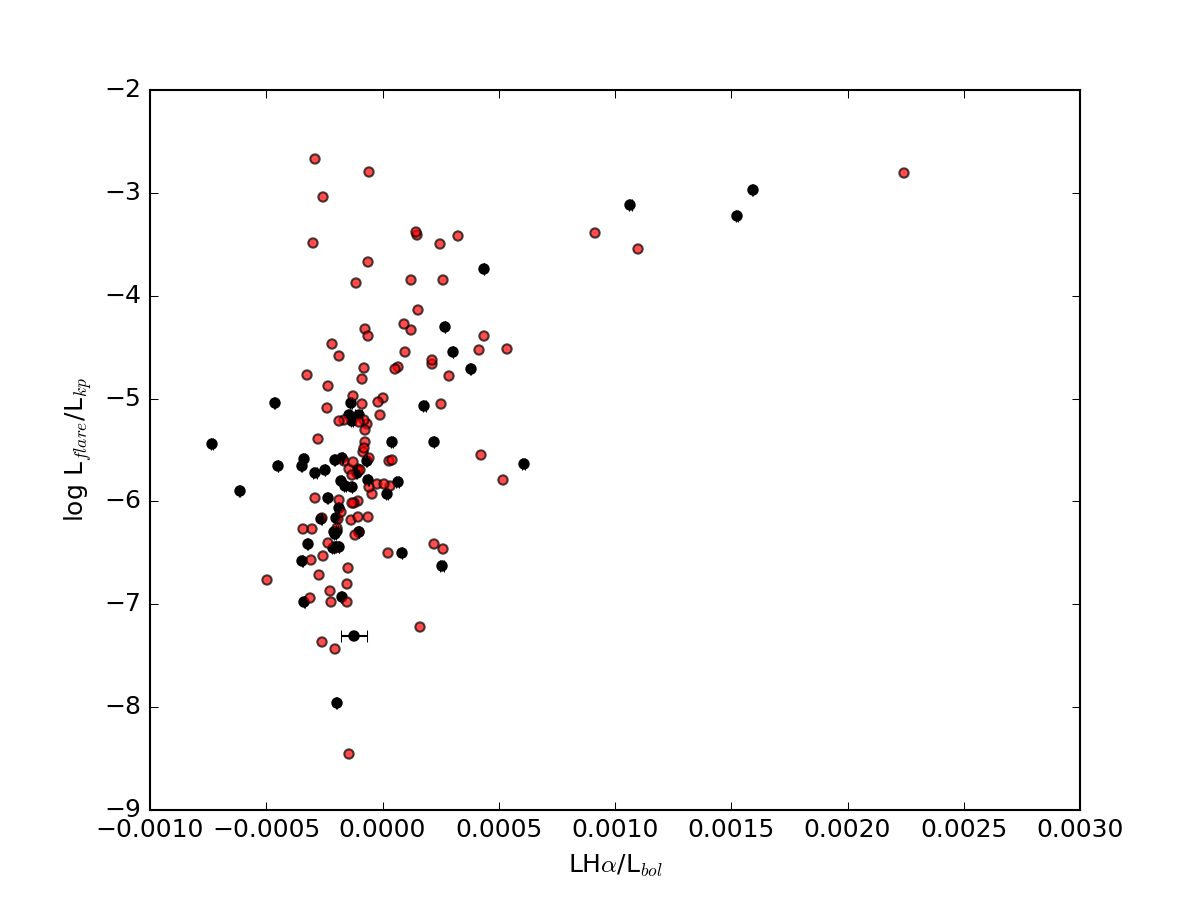
\includegraphics[width=3.5in]{figures/flare_vs_lhalbol.png}
\caption{
H$\alpha$ vs flare energy
}
\label{fig:halpha}
\end{figure}



%%%%%%%%%%%%%%%%%%%%%%%%%%%%%%
\section{Discussion}

this is the first time a direct connection between stellar flare energy and other traditional magnetic activity indicators has been determined, tying the occurrence of flares on small size scales to the total chromospheric activity of the star.


%%%%%%%%%%%%%%%%%
\acknowledgments
JRAD is supported by an NSF Astronomy and Astrophysics Postdoctoral Fellowship under award AST-1501418.
Kepler was competitively selected as the tenth Discovery mission. Funding for this mission is provided by NASA�s Science Mission Directorate.



\bibliography{/Users/davenpj3/Dropbox/references}


\end{document}
